\section{\textsc{Mathematical Frameworks}}
\hrule height 1pt
\vspace*{5pt}

\subsection{\textsc{come up with title}}
\vspace*{-10pt}
We know that every position on a map corresponds to a unique point on
Earth. In mathematical language, this is a bijection (one-to-one and onto mapping)
 - when a function is both an injection and surjection. 
\begin{definition}{Bijection (Libretexts, 2021)}
    Let $f:A\mapsto B$
    
    \begin{center}
        \textbf{Injection (one-to-one)} - for all $x_1, x_2 \in A$, if $x_1\neq x_2$, then $f(x_1)\neq f(x_2)$\\
        \textbf{Surjection (onto)} - for every $y\in B$, there exists $x\in A$ such that $f(x)=y$\\
    \end{center}

    A bijection function holds both of these properties.
\end{definition}
It helps to think of the map and the Earth as two sets containing points, where the function 
$f$ maps each point on the Earth (set $A$) to a unique point on the map (set $B$) because it 
formalizes the intuitive concept of a perfect map. Injection ensures two distinct places on Earth
cannot merge into one point on the map while surjection guarentees every map location corresponds to
a real place on Earth. 

It is also necessary to define the notion of \textit{distance}, as ambiguity may arise without a clear 
specification. For instance, distance could refer to the shortest path through ambient space (the chord 
passing through the Earth's interior), the straight-line or ``as-the-crow-flies" distance, or the actual travel 
distance along roads between two locations. The distance which cartographers will deal with is called the 
intrinsic or geodesic distance (Ozuch, 2024). 
\begin{definition}{Geodesic distances}
    Given a surface $\Sigma$ embedded in ambient space, if $A$ and $B$ are points of $S$, we can then consider 
    the infinite amount of the lengths of curves included in $\Sigma$ joining these two points (dashed lines). 
    \begin{center}
        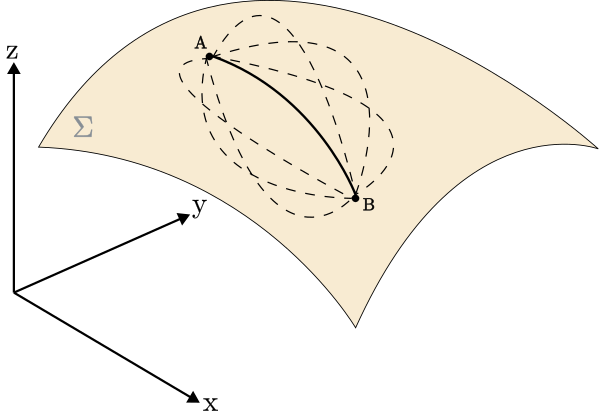
\includegraphics[width=0.55\linewidth]
        {figures/distance.png}
    \end{center}
    Out of these curves, the one with the minimum length (solid line) is the intrinsic or geodesic distance on the surface. 
    This will be denoted as $d(A,B)$.
\end{definition}
Having established the necessary definitions, we can now mathematically describe what a faithful map is: a map that
preserves all distances between any pair of points, up to a scale change. This property is called \textit{isometry} 
- a challenge that many cartographers try to achieve for centuries (Wolfram, 2025). 

\pagebreak
\subsection{\textsc{Gaussian Curvature}}
\vspace*{-10pt}
Gauss curvature, commonly denoted as $k$, is the product of the minimal and maximal curvatures of geodesics starting from a point.

<insert diagram>

The precise mathematical definition of curvature is too complicated beyond the scope of this Extended Essay, so I will 
describe the intuitive understanding of it instead. Construct a tangent plane at a point on the surface; if:
\begin{itemize}
    \item the surface is contained on one side of its tangent plane will have positive curvature.
    \item the surface is intersected with its tangent plane will have negative curvature.
    \item the surface with one of its segments contained in the tangent plane will have 0 curvature. 
\end{itemize}

Another way to understand curvature is by comparing the properties of objects on that surface. One such comparison tool is
the Toponogov's Theorem.

\pagebreak
\subsection{\textsc{Parametric Surfaces}}
\vspace*{-10pt}
A surface in three-dimensional space is often most effectively 
described using a parametric representation. In this framework, a 
surface is defined by a vector-valued function
\begin{equation}
    \vec{r}(u,v)=x(u,v)\vec{i} + y(u,v)\vec{j} + z(u,v)\vec{k}
\end{equation}
where $u$ and $v$ are independent parameters that vary over a 
two-dimensional region $D$ in the $uv$-plane. The set of all such position 
vectors forms the parametric surface $S$ (Dawkins, 2024).

Unlike implicit surfaces defined by equations of the form $F(x,y,z)=0$, parametric
surfaces allow for the direct generation of points and the computation of geometric
properties such as tangent vectors through partial derivatives, which will later 
on prove itself useful in the context of cartography.

If we express the two parameters $u$ and $v$ as a function of another variable
$t$, then by applying the chain rule to $\vec{r}(u(t),v(t))$ with respect to 
$t$, we get:
\begin{equation}
    \frac{d\vec{r}}{dt}=\frac{\partial \vec{r}}{\partial u}\frac{du}{dt}+\frac{\partial \vec{r}}{\partial v}\frac{dv}{dt}
\end{equation}
This derivative represents the tangent to the curve formed by $u(t)$ and $v(t)$ 
(Patrikalakis et al., 2009).

Another important property of surfaces, particularly relevant in cartography, 
is the notion of smoothness. Depending on the desired level of accuracy, the 
Earth's surface may be modeled in various ways: as a perfect sphere, an oblate 
spheroid, or a more complex geoid that represents mean sea level variations. 
Regardless of the chosen model, a key geometric feature of such surfaces is 
that, when observed at an infinitesimally small scale, they resemble a flat 
plane. In other words, the surface is locally planar, a property that 
characterizes it as smooth (Ozuch, 2024).

As mentioned in the introduction, we will model the Earth as a perfect unit sphere
due to the limited scope of this Extended Essay. Let $\phi$ and $\lambda$ be
the longitude and latitude of the Earth, acting as parameters of the surface, 
and let $M(\phi,\lambda)$ be a point on the Earth's surface. 

\begin{wrapfigure}{l}{0.45\linewidth}
    \centering
    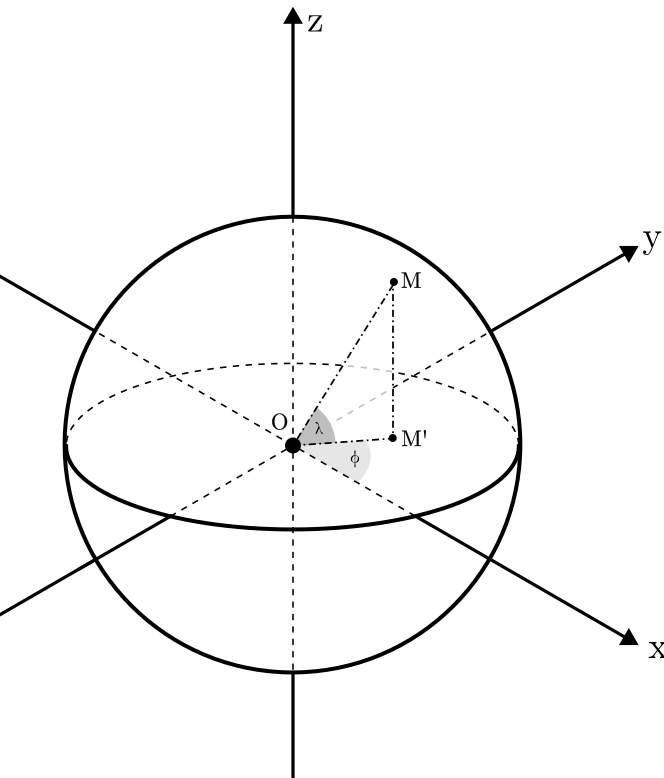
\includegraphics[width=0.75\linewidth]
    {figures/earth unit sphere.png}
    \caption{Earth as a sphere centered at $(0,0,0)$}
    \label{fig:figure2}
\end{wrapfigure}

Fix the center of the spherical Earth at the origin of the Cartesian coordinate $(0,0,0)$, with
the poles aligning with the $z$-axis. Let $M'$ be the projection of point $M$ onto
the $xy$-plane in 3D Cartesian space. We can see that the $z$-coordinate of $M$
would be
\begin{equation*}
    z= MM'=\sin\lambda
\end{equation*}
To find the $x$ and $y$-coordinate of point $M$, we first find the coordinate in terms of $OM'$ using
trigonometry and then substitute $OM'=\cos\lambda$, obtaining
\begin{align*}
    x&=OM'\cos\phi=\cos\lambda\cos\phi\\
    y&=OM'\sin\phi=\cos\lambda\sin\phi
\end{align*}
Thus, the parametric equation of the model Earth is
\begin{align}
    \vec{r}(\phi,\lambda)=\cos\lambda\cos\phi\vec{i} + \cos\lambda\sin\phi\vec{j} + \sin\lambda\vec{k}
\end{align}